\documentclass[11pt,letterpaper]{article}
\usepackage[rmargin=1.5in, left=1in]{geometry}
\usepackage[utf8]{inputenc}
\usepackage[T1]{fontenc}
\usepackage{hyperref}
\renewcommand{\familydefault}{\sfdefault}
\usepackage{helvet}
\pagestyle{empty}
\usepackage[kerning=true]{microtype}
\usepackage{parskip}
\usepackage{sansmath}
\usepackage{graphicx}
\usepackage{sidecap}  
\sidecaptionvpos{figure}{c}
\usepackage{float}
\usepackage{color, soul}
\usepackage{fancyhdr}
\usepackage{marginnote}
\usepackage{algorithm}
\usepackage{algpseudocode}
\pagestyle{fancy}
% Feel free to use additional packages for glosses, figures, whatnot.
\usepackage[dvipsnames]{xcolor}
\newcommand{\train}[1]{\textcolor{BurntOrange}{[Train: #1]}}
\newcommand{\unclear}[1]{\textcolor{Cerulean}{[Unclear: #1]}}
\newcommand{\timing}[1]{\textcolor{ForestGreen}{[Time: #1]}}
% The next bit is for reserving sufficient space for authors,
% affiliations, and e-mail address.  No need to change for initial
% anonymous version.  For the final version, replace the
%\toggletrue{anonymous} %with \togglefalse{anonymous} to de-anonymize.
\usepackage{etoolbox}
\newtoggle{anonymous}
\togglefalse{anonymous}

\renewcommand{\title}[1]{\textbf{#1}\\}
\newcommand{\authors}[1]{\iftoggle{anonymous}{\phantom{#1}}{#1}\\}
\newcommand{\email}[1]{\iftoggle{anonymous}{\phantom{#1}}{#1}}

\begin{document}

% First page:

% Insert title, authors, affiliations, and e-mail address in the next three lines:

\title{Investigating language drift in multi-agent communication about natural images: MSc Thesis Proposal V2 \newline}
\authors{By Polina Tsvilodub, \textit{February 16th 2022}}

The following proposal refines the topic for my MSc thesis. More specifically, the thesis will focus on identifying and potentially counteracting language drift which arises in multi-agent communication experiments employing natural language as the communication protocol. The experiments will be based on the MS COCO Captions dataset which two agents will communicate about in a reference game setting \cite{chen2015microsoft, lazaridou2016multi}.

Along with this outline, I put together a thesis schedule, describing the time frame of the project. In this proposal, all work \textit{milestones} are enumerated (preceded by an \textit{M}) in the order I will work on them. You can find respective milestones and corresponding work step numbers on the right of the text. The milestones are referenced in the schedule. This outline is structured according to the suggested flow of the thesis (i.e., from introduction to conclusion).  
Additionally, a \textit{pseudo algorithm} of the experiment is provided at the end of the write-up. Comments in \timing{green} highlight the aspects that I assume might be time intensive or which would have an effect on project timing, while comments in \unclear{blue} highlight design decisions which I am unsure about.

\underline{Most important dates:}
\begin{itemize}
	\item Register thesis by May 23rd 2022 \marginnote{M7.1}
	\item Finish thesis draft by August 1st 2022 \marginnote{M7.2}
	\item Submit thesis by August 31st 2022 \marginnote{M7.4}
\end{itemize}

\subsection*{Outline:}

\begin{enumerate}	
\item \underline{Introduction \& Theoretical Background on Multi-Agent Communication}

This section will cover the motivation of current work, \marginnote{Steps 2, 5\\M2.1, M5.1} as well as review related work in the area of multi-agent communication. 

\begin{itemize}
	\item The area of multi-agent communication has gained increased popularity (e.g., \cite{lazaridou2020emergent}). This thesis particularly focuses on multi-agent communication experiments employing communication in natural language (i.e., English) (e.g., \cite{andreas2016reasoning, mao2016generation, lazaridou2020multi, gupta2021dynamic}). 
	\item The proposed experiment will use a reference game setting, so the relavant background as well as related multi-agent reference game experiments will be reviewed (e.g., \cite{lazaridou2016multi}). Other tasks used in multi-agent communication experiments will also be reviewed (e.g., \cite{jaques2019social}).
	\item The thesis will take multi-agent communication one stop closer towards real-world applications by using real images from the \textbf{MS COCO Captions dataset} \cite{chen2015microsoft}. This dataset features photographic images alongside with five manually annotated captions per image, assigned categories (80 in the entire dataset), object bounding boxes, as well as other features like whether the image is crowded or not. 
	\item Previous work either uses such a dataset (e.g., \cite{havrylov2017emergence}), or focuses on using natural language. Some experiments combine both by using single natural language labels for the images (e.g., \cite{lazaridou2016multi}), but full captions have not been used yet.
	\item Therefore, current work will focus in combining natural images and natural language, while particularly zooming in on the quality of the language. 	
	
\end{itemize}

\item \underline{Theoretical Background on Image Captioning}

This chapter will cover necessary background in neural image captioning. \marginnote{Step 2\\ M2.1} 
 
\begin{itemize}
	\item The experiments conducted in the thesis will use the overall architecture proposed by \cite{lazaridou2020multi}. That is, the captioning module will consist of an LSTM cell, as proposed by \cite{vinyals2015show}, while the image embedding module will be based on a pretrained ResNet-50 \cite{he2016deep} (more details below). 
	\item This chapter will review different approaches to image captioning (e.g., \cite{karpathy2015deep, vinyals2015show, vedantam2017context, kim2021vilt}). Other related tasks like visual question answering will be mentioned, as well.
	\item Both multi-agent communication as well as image captioning might be prone to \textit{language drift}, i.e., the decreasing quality and intelligibility of natural language as task-specific training proceeds. However, this issue hasn't received much attention in the literature (but see e.g., \cite{lee2019countering}), so current work will specifically focus on language drift. The next chapter outlines the experimental setting, followed by an in-depth discussion of language drift in Chapter 4. 
\end{itemize}

\item \underline{Own Experiment}

In order to investigate language drift,\marginnote{Steps 1, 3, 4} several multi-agent reference game experiments would be conducted. Their design will closely follow \cite{lazaridou2020multi}. This section will describe the dataset, experimental set up and training procedure. A more formal summary can be found under Algorithm \ref{ref-game-alg}. \train{Steps in orange} indicate parts of the experiment which I assume to require training.  Preferably, the experiments would be implemented using TensorFlow \cite{abadi2016tensorflow}. First, ``minimal viable product'' (MVP) \marginnote{M1.4}versions of the models would be implemented and trained on a small scale locally, to ensure that the architecture works. Following that the models would be trained at full scale. \marginnote{M3.2}

\begin{itemize}
	\item In the reference game, two neural agents will receive pairs of images, and the speaker agent's task will be to produce a message identifying the target image among the two. The listener agent's task will be, given the speaker's message, to pick the correct image among the two. This reference game set up allows to introduce a cognitively plausible task objective---producing a maximally discriminative caption for the target image, highlighting its differences to the distractor image (\cite{andreas2016reasoning, dai2017contrastive, vedantam2017context, nie2020pragmatic}). 
	\item Each agent will consist of two modules: the visual module which produces a feature vector given raw images, and the language module which produces or decodes messages (i.e., image captions), respectively. 
	Following \cite{lazaridou2020multi}, the visual encoding modules for both agents will consist of pre-trained ResNet-50 modules (available both in TensorFlow and Pytorch, \cite{he2016deep}). Following \cite{vinyals2015show}, the language module of the speaker will consist of an LSTM which will produce messages conditioned on the image embeddings. KL regularization will be used. 
	\item \timing{The speaker will be trained to produce discriminative captions by using a ``multi-task'' approach where the agent is optimized to produce both structurally fluent and functionally correct (i.e., discriminative) captions \cite{lazaridou2020multi}.} (see Alg. \ref{ref-game-alg}) This architecture might be prone to language drift, making it a good avenue for investigating this phenomenon.
	\unclear{I am not sure if this is the optimal loss / architecture to use. An alternative would be to use a pretrained captioning module, only fine-tuning it on the task.}
	\item \timing{Two versions} of this experiment will be conducted.\marginnote{M1.5, M3.1} The first version would use \textbf{random image pairs} as target and distractor during training. Because the dataset consists of images belonging to 80 different categories, images from different categories might feature completely different scenes, making detailed descriptions superfluous. This first experiment will serve as a baseline, and to investigate whether the captions remain short and reference minimal necessary features, or if the speaker overgenerates. Furthermore, this experiment will be a baseline for checking if the desired set up (i.e., the dataset and natural language) works at all. 
	\item The second version would use \textbf{within-category} target and distractor image pairs. To group the images, image pairs would be constructed by using images for which at least two category labels are the same (each image has several category annotations provided by each of the annotators which might vary). Using more similar images would, ideally, pressure the speaker to produce more detailed, longer captions. This second experiment might give the room necessary for investigating language drift. 
	\item The two experiment versions would be compared with respect to referential success of the agents in order to validate the experiment. Descriptive analyses will also be conducted, like comparing average caption lengths for the two experiments. The caption complexity could also be compared as a function of target/distractor similarity (computed, e.g., \unclear{as cosine similarity between the image embeddings}).
	\item \timing{For both experiments, the idea would be to use roughly a quarter of the categories (i.e, 20), yielding around 70.000 images.}\marginnote{M1.3} One could use about 5-10\% of images in each category used for training as validation data (around 3.500 images in total). Two test splits could be created: one split could contain images with categories partially observed during training (easy split), while images from, e.g., five unseen categories can be used as a difficult test split. It is hard to consider the categories as clearcut ``novel'', though, because many images have different category labels assigned to them. This issue could be tackled by only using images with, e.g., at least three out of five (non)overlapping categories.  
	\item \unclear{Maximal message length could be set to the maximal caption length appearing in the dataset. The vocabulary could consist of all the tokens appearing in the entire dataset.}  
	\item \unclear{Potentially, a different model as a baseline could be useful.}
	\item \unclear{For both experiments, the models would be trained until convergence.}
\end{itemize}

\item \underline{Analysing Language Drift}

This\marginnote{Steps 1, 3, 4} thesis aims to compare state-of-the-art language drift metrics and to attempt to develop a novel metric. Therefore, this section will review existing language drift metrics (e.g., \cite{lazaridou2020multi, lu2020countering}), provide theoretical background for the proposed metrics and analysis, and present several approaches to developing a new metric. 
Existing drift metrics which are applicable to the proposed experiment would all be computed for both experiments. More specifically, they could be computed both during the training (e.g., every 50 training steps) to assess the dynamics of language development, as well as for the trained models on the test split. A more formal overview of the required models can be found under Algorithm \ref{alg:drift}.
Existing language drift metrics include:
\begin{enumerate}
	\item Structural / syntactic language drift: log probability of the generated message $m$ under a pre-trained unconditional language model $P(m)$ \cite{lazaridou2020multi}
	\item Semantic language drift: conditional log probability $P(m|i)$ of the generated message $m$ given the image $i$. Another measure includes the n-gram overlap of generated messages and the ground-truth captions (ignoring stopwords) \cite{lazaridou2020multi}. Semantic drift is also addressed by \cite{lee2019countering, lu2020countering}, but their approaches rather propose specific training methods than measures for identifying language drift, so their proposals wouldn't be considered here.
	In alternative framings, semantic drift has been measured as the difference between the message semantics and the action taken by the receiver agent \cite{jacob2021multitasking}.
	\item Pragmatic language drift: \cite{lazaridou2020multi} assess this drift as referential failure in absense of structural or semantic drift by comparing human and listener agent referential success given a model which only reranks ground-truth captions. Given that the currently proposed experiment won't have human data, this kind of drift will have to be assessed differently. Although the proposed approach has the advantage of being task-agnostic, in this work, I would propose to focus on a referential task drift which I referred to as \textit{functional} drift. 
\end{enumerate}
Similar to the experimental models,\marginnote{M1.7} first, MVPs of the models for language drift analysis would be implemented and tested, before training them full-scale.\marginnote{M3.2}

A novel metric would focus on evaluating both structural and \textbf{functional drift} of the produced expressions. In this context, funtional drift would refer to the deterioration of language which would make the referential task impossible for humans (e.g., leaving out critical content words). Structural drift, in contrast, might involve mixing up the word order, which nevertheless wouldn't hinder the referential task, if distinctive content words are still present. For instance, the caption ``A plate food with'' would exemplify functional drift, while the caption ``A plate red food with'' wouldn't, if Figure \ref{fig:screenshot003} was the target image and Figure \ref{fig:screenshot002} was the distractor. 

\begin{figure}
	\centering
	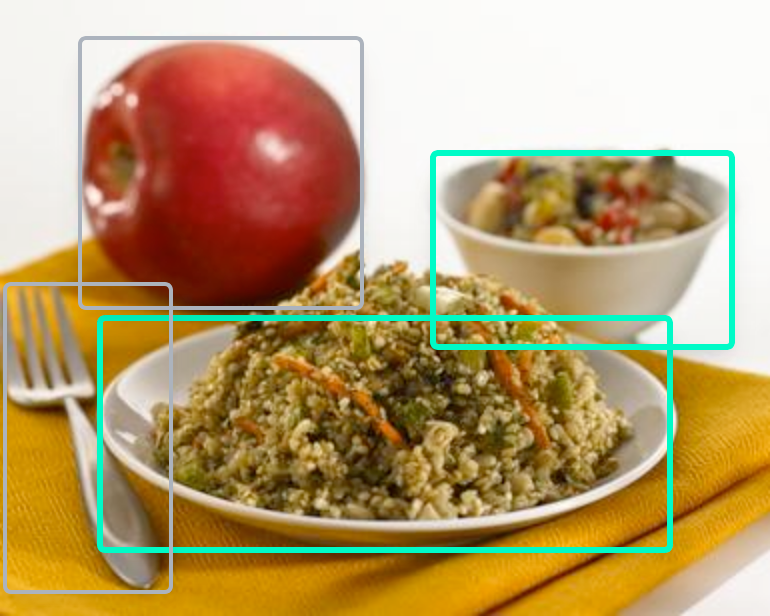
\includegraphics[width=0.5\linewidth]{images/screenshot002.png}
	\caption{Example image from the MS Coco Captions dataset. Example caption: ``The plate is piled with rice next to a whole apple.''. Assigned categories: [fork, bowl, apple, bowl]}
	\label{fig:screenshot002}
\end{figure}
\begin{figure}
	\centering
	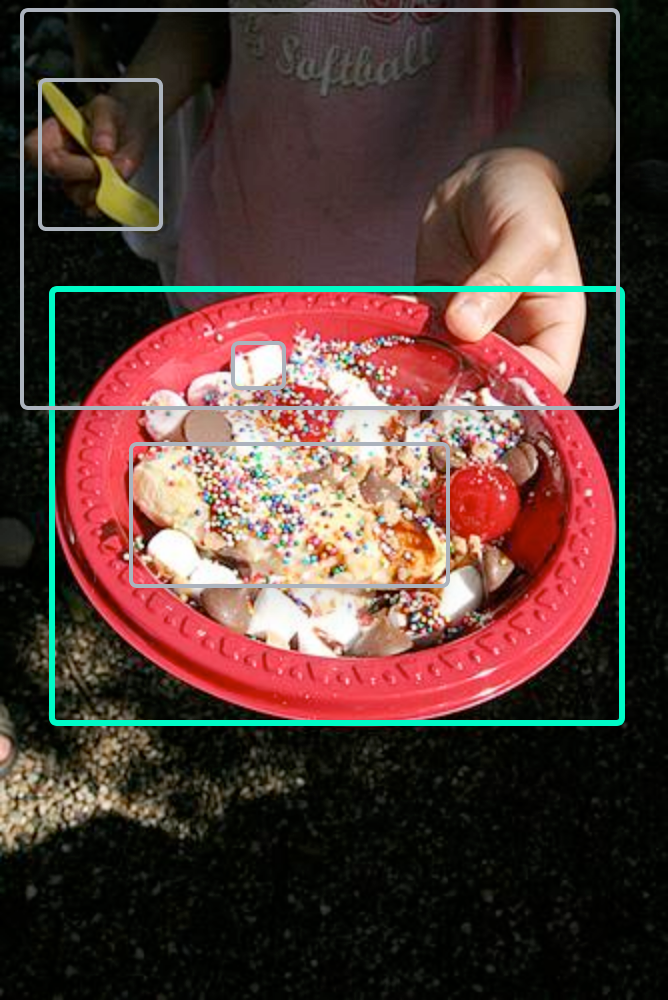
\includegraphics[width=0.3\linewidth]{images/screenshot003.png}
	\caption{Example image from the MS Coco Captions dataset. Example caption: ``A person holding a red bowl filled with cake.''. Assigned categories: [person, spoon, bowl, banana, banana]}
	\label{fig:screenshot003}
\end{figure}

Different approaches to developing such a metric could be taken in the thesis. 
\begin{enumerate}
	\item One idea for identifying functional language drift which would also be stable against compositional alternations within the caption would be to compute the word overlap between the generated captions and the target and distractor ground truth captions, respectively. From a functional perspective, an optimal generated target caption would maximize the overlap with the target ground truth, while minimizing the overlap with the distractor ground truth. This idea is related to the omission score suggested by \cite{havrylov2017emergence}. \unclear{This descriptive metric might possibly even be converted into a version of a contrastive loss for training the speaker agent (cf. \cite{andreas2016reasoning, gunel2020supervised}).}
	\item Alternatively, the idea described above could be formalized by computing the cosine similarity between the caption embeddings instead of word overlap scores. 
	\item A more structured approach to identifying whether critical discrimnative components have been captured in the caption might be to consider the labeled objects in the two images, identify the ones that are only present in the target image, and perform image patch to caption alignment, as proposed by \cite{karpathy2015deep}. Higher alignment scores would indicate more discriminative captions. \unclear{However, the availability of the model and the usefulness of the approach are not completely clear, as the similarity of images even within MS Coco Captions categories might be quite variable.}
	\item Finally,\marginnote{M1.6, M3.2} we discussed the idea to measure the drift as the similarity between the original image and an image generated by a pretrained text-to-image model given the generated caption. Some text-to-image architectures include DALL-E, StackGAN++ or other models \cite{ramesh2021zero, zhang2018stackgan++, zhou2021lafite}. \timing{However, it seems rather difficult to find models, pretrained on our dataset. Example sources for other datasets might be \url{https://tinyurl.com/y4pz7ymz} or \url{https://github.com/ShanHaoYu/Text2Image}. Although comprehensive guides to training these models exist, computational demands for this task might be rather cosmic.}
	 \unclear{Furthermore, a similarity metric for the original and generated image would be necessary. One could potentially compare embeddings of these images extracted by the ResNet module via cosine similarity, but the interpretability of such a comparison might be unclear}.  
	 \item Based on this idea, \timing{a different approach to training could be considered,} whereby an image could be generated from the ground truth caption as an intermediate representation (cf. \cite{lee2019countering}). \unclear{Specifics of the architecture would have to be determined, provided the availability of a text-to-image model.}  
\end{enumerate}
If feasible,\marginnote{M3.3, M4.1} all these approaches could be tested in similar way as the exisiting metrics (i.e., during training and on the test split), and compared with respect to their accuracy and functional adequacy by manual inspection of caption samples. 

\item \underline{Conclusion \& Discussion}

This section will summarize the work,\marginnote{Step 6} outline its contributions and limitations. More specifically, the generalizability of the considered drift metrics to different tasks and different datasets will be discussed. The susceptibility of the metrics to design decisions regarding the experimental set up, as well as properties of the dataset will be covered. Depending on the results, the reasons for failure or improvements will be discussed. Finally, an outlook to directions for future work will be given.

\begin{algorithm}[h]
	\caption{Basic reference game set up}
	\label{ref-game-alg}
	\begin{algorithmic}
		\State $|images| = n$
		\State $|caption_i| = t $ for the caption of the $i-$th image
		\State $f$: LSTM network		
		\State $h_m:  $ LSTM hidden state
		\State $x_m$: $m$-th input token to the LSTM, $m \in {1,...,t }$
		\State $y_m$: $m$-th ouput token of the LSTM 
		\For{image $ i$ in $[1, n]$}
			\State \underline{\textbf{Speaker agent:}}
				\State target image embedding $u_i \gets $ ResNet-50 
				\While{$m +1<$ max caption length or $y_{m+1} \neq$ STOP }
				\For{caption token $x_m$ in $[1, t]$ of image $i$ }
					\State maximize $log P(x_m | x_0...x_{m-1}, u_i) = \sum_{m=0}^{m-1} log P(x_{m-1}|x_0...x_{m-1}, u_i)$
					\State \unclear{$h_0 \gets u$}
					\State \train{$h_{m+1} = f(h_m, [x_m, u_i])$; 3 gates;} \unclear{concatenated $x_m$ and $u_i$}
					\State \train{$y_{m+1} = Softmax(h_m)$} over all words in vocabulary 
				\EndFor	
				\EndWhile
				\State Loss speaker: \\ $L_S= \lambda_fL^{functional} + \lambda_s L^{structural} = -r^L(caption, u, i)\sum_{m=0}^{t}log P_{\theta_S^{LSTM}}(caption^m|caption^{<m}, [u_i, u_d]) + \lambda_s \sum_{m=0}^{t}log P_{\theta_S^{LSTM}}(caption^m|caption^{<m}, u_i) +$\texttt{ KL-regularisation} where $t$ is longest caption in the dataset, updating $L^{functional}$ via \texttt{reinforce}\\
				
			\State \underline{\textbf{Listener agent:}}
				\State target image embedding $u_i \gets $ ResNet-50 
				\State distractor image embedding $u_d \gets$ ResNet-50 (sampled either at random or within-category of the target)
				\For{token $y_m$ in $[1, t]$ of received message $y$} 
					\State \train{$v_m = f(y_m)$  }
				\EndFor	
				\State \unclear{caption embedding: $v = maxpool(v_1...v_t)$ \cite{conneau-EtAl:2017:EMNLP2017}}
				\State target = $max_{i, d} (v \times u_i, v \times u_d)$ where $\times$ is the dot product similarity
				\State Loss listener: \\
				$L_L = -(target \; log(P(i)) + (1-target)log(1-P(i)))$ \\	

			\State \textbf{Loss:}
			\If{target identified correcly}
			\State Reward $r^L= 1$ 
			\Else
			\State Reward $r^L= -1$ 
			\EndIf	
			
			\unclear{$ L = L_S + L_L$ (cf. \cite{lee2019countering}).
			Only LSTM and projection components are trainable, although e.g., \cite{vinyals2015show} also update the top CNN layer.}

		\EndFor
		
	\end{algorithmic}
\end{algorithm}

\begin{algorithm}[h]
	\caption{Set up of models required for drift metrics}
	\label{alg:drift}
	\begin{algorithmic}
		\State \textbf{Semantic drift: Pretrained language model}
		\State Compute perplexity of the captions under a pretrained model, e.g., GPT-2 provided by the \texttt{huggingface} library \\
		\State \textbf{Structural drift: Image captioning model}
		\State \train{LSTM trained with caption log likelihood objective only, as proposed by \cite{vinyals2015show}}, such that the architecture maximally closely matches experimental architecture in Algorithm \ref{ref-game-alg}. The same training split would be used. \\
		Loss: $L = - \sum_{m=0}^{t}log P_m(x_m)$ for a caption of length $t$. \unclear{The same components of the model should be trainable as in Alg. \ref{ref-game-alg}. The availability of a pretrained model will also be investigated} \\
		\State \textbf{Functional drift: \unclear{Text-to-image}}
		\State \train{The pretrained model by \url{https://github.com/ShanHaoYu/Text2Image} is implemented in TensorFlow, which would allow to easily include it in the pipeline. However, it is unclear on which dataset it is trained. It might potentially need finetuning, since the original implementation by \cite{zhang2018stackgan++} also trains on different datasets than MS Coco.}
	\end{algorithmic}
\end{algorithm}

\end{enumerate}

 
\bibliographystyle{apalike}
\bibliography{tsvilodub_msc_thesis_proposal.bib}
\end{document}
